\documentclass[a4paper, oneside, 12pt, onecolumn]{article}
\usepackage{settings}
\usepackage{listings}
\usepackage{lscape}
\definecolor{light-gray}{gray}{0.95} 
\RequirePackage[framemethod=TikZ]{mdframed} % Required for creating the theorem, definition, exercise and corollary boxes


\mdfdefinestyle{exampledefault}{
  rightline=true,
  %frametitlerule=true,
  %frametitlefont=\ttfamily,
  %frametitlerulecolor=black,
  %frametitlebackgroundcolor=lightgray,
  %frametitlerulewidth=2pt,
  backgroundcolor=light-gray,
  roundcorner=5pt,
  %outerlinecolor=blue!70!black,
  %outerlinewidth=2,
  leftmargin=20,
  rightmargin=20,
  ntheorem=true,
  innerleftmargin=15, 
  innertopmargin=1,
  innerbottommargin=1,
  outerlinewidth=1,
  linecolor=light-gray
}
\mdfsetup{
  frametitlealignment=\flushleft
}

\lstdefinestyle{customc}{
  %backgroundcolor = \color{lightgray},
  belowcaptionskip=1.1\baselineskip,
  breaklines=true,
  %frame=L,
  %xleftmargin=\parindent,
  language=C,
  showstringspaces=false,
  basicstyle=\footnotesize\ttfamily,
  keywordstyle=\bfseries\color{green!40!black},
  commentstyle=\itshape\color{purple!40!black},
  identifierstyle=\color{blue},
  stringstyle=\color{orange},
}

\lstset{escapechar=^,style=customc}

\captionsetup[lstlisting] { 
  font={normalsize,tt},
  justification=raggedright,
  singlelinecheck=false
}

%\geometry{a4paper,top=2.5cm,bottom=4.6cm,left=1.5cm,right=1.5cm,columnsep=15pt,heightrounded}


%biber: rm -rf `biber --cache`

\newcommand{\pc}{\texttt{pandoraCosmic}\xspace}
\newcommand{\pn}{\texttt{pandoraNu}\xspace}
\newcommand{\ls}{\texttt{LArSoft}\xspace}
\newcommand{\lars}{\texttt{LArSoft}\xspace}
\newcommand{\extbnb}{\texttt{EXTBNB}\xspace}
\newcommand{\bnbon}{\texttt{BNBON}\xspace}
\newcommand{\bnbcosmic}{\texttt{BNBCosmic}\xspace}

%+++++++++++++++++  TITLE
%\pretitle{\begin{center}\Huge\bfseries} % Article title formatting
%\posttitle{\end{center}} % Article title closing formatting
\title{How to Normalise Data and MC} % Article title
\author{%
\textsc{Marco Del Tutto}\thanks{\mail{marco.deltutto@physics.ox.ac.uk}} \\ % Your name
%\normalsize Department of Physics, University of Oxford,\\ 
%\normalsize Oxford OX1 3RH, United Kingdom \\[1ex] % Your institution
%\normalsize Representing the \uB Collaboration
%%\normalsize \href{mailto:marco.deltutto@physics.ox.ac.uk}{marco.deltutto@physics.ox.ac.uk} % Your email address
}
\date{\today} % Leave empty to omit a date
\renewcommand{\maketitlehookd}{%
\begin{abstract}
This note describes how the calculate the normalisation between the on-beam and off-beam samples. It also shows how to normalise MC events to be compared to data.\\
Thanks to Nicolò Foppiani\thanks{\mail{nicolofoppiani@g.harvard.edu}} for adding NuMI-related instructions. 
\end{abstract}
}
%+++++++++++++++++






\begin{document}

\maketitle

%\listoftodos

%\tableofcontents


%\newpage

\section{Data Normalisation}

The on-beam sample is never scaled, but the off-beam sample is scaled to match the POT exposure of the on-beam one.

The number of POTs and triggers for a given data sample can be retrieved thanks to a tool developed by Zarko Pavlovich, which allows to read these information by providing the list of runs and subruns one has run over. The POT information are stored per subrun. To avoid considering subruns in files that fail the grid processing, one should generate a list of run and subruns only for the files that have been output by the grid, and with this list can query the tool for the POT information. The files in the official MicroBooNE datasets have an optical filter applied. Nevertheless, this is not an issue for the POT counting as the subrun information is stored in the art-root files even if no events in a certain subrun pass the filter.

There are two ways to get the POTs for the files one has run over. One can either create a SAM definition for those files, and then query Zarko's script via\\

\texttt{/uboone/app/users/zarko/getDataInfo.py -v2 your\_sam\_definition\_name}\\

or one can dump the run and subrun numbers with a \ls module (for example the module used for the analysis). See section \ref{sec:dump} on information on how to dump these numbers. In this case one would call Zarko's script with a text file that contains the run and subrun numbers:\\

\texttt{/uboone/app/users/zarko/getDataInfo.py -v2 \\-\/-run-subrun-list runsubrun\_list.txt}\\

The script will show several variables. One should run this script for both data \bnbon and \extbnb. When running over \bnbon, one should look at the variable \texttt{tor860\_wcut}, which gives the number of POTs corresponding to the number of events one has run over, $N_t^\text{ON}$. The variable \texttt{E1DCNT\_wcut} gives the number of issued triggers, $N_t^\text{ON}$. \texttt{\_wcut} means with quality cuts applied.

When running over \extbnb, one should only look at \texttt{EXT}, which gives the number of triggers, $N_t^\text{OFF}$. 

The normalisation of off-beam to on-beam data is done by normalising to the same amount of spills/pulses received \emph{before} the software trigger was applied.

To normalise the \extbnb sample to the \bnbon sample, one should weight every event in \extbnb with a factor of $N_t^\text{ON}/N_t^\text{OFF}$. In this way both samples will be normalised to an exposure of $N_\text{POT}$ POTs.

If you are dealing with NuMI data instead, things are pretty similar, except for two caveats:
\begin{itemize}
    \item The name of the variables you need to retrieve from Zarko's tool are different
    \item The NuMI external trigger is prescaled. This means that, instead of storing all the events that fired a trigger, only one out of a certain prescale factor is stored. The prescale factor that has been applied varies on a run by run basis. To count properly the number of issued triggers you need to scale each event for the proper prescale factor.
\end{itemize}

By running this line, you would pick a modifided version of Zarko's tool which takes into account the prescale factor:\\
\texttt{/uboone/app/users/zarko/prescale/getDataInfo.py -v2 -\/-prescale\\ -\/-run-subrun-list runsubrun\_list.txt \\-f EXT:EA9CNT\_wcut:tortgt\_wcut:tor101\_wcut }\\

To summarize here is a table of the variables you need:

\begin{table}[!h]
\begin{tabular}{l|l|l}
Variable            & BNB                                    & NuMI \\
\hline
Beam ON - $N POT$  & \texttt{tor860\_wcut} & \texttt{tortgt\_wcut}\\
Beam ON - $N_t^\text{ON}$  & \texttt{E1DCNT\_wcut} & \texttt{EA9CNT\_wcut}\\
Beam OFF - $N_t^\text{OFF}$ & \texttt{EXT}          & \texttt{EXT\_NUMIwin\_FEMBeamTriggerAlgo}
\end{tabular}
\end{table}

\subsection{Motivation}

This Section describes why we are normalising beam-off data to beam-on data using the number of triggers.
On average, our simulation predicts one neutrino interaction every $\sim 600$ beam spills. This means that if we take 600 on-beam data events, they will contain, on average, 599 events with cosmics only, and only one event with cosmics and one neutrino interaction. The normalisation of off-beam to on-beam data is done by normalising to the same amount of spills/pulses received \emph{before} the software trigger was applied. Once this normalisation is applied, one may think that this completely removes the cosmic contamination in the final selected sample, and one remains with a distribution of neutrino candidates only. Unfortunately this is not true, as when the selection runs over the event with a neutrino interaction, may mistakenly select a cosmic instead. Although the number of selected events will reflect the selected number of neutrino interactions, the distribution will not reflect completely the properties of the selected neutrinos, but will partially contain a cosmic contamination. This is why the simulation that we use contains neutrinos overlaid with cosmic interactions. At this point, the best option would be to remove 599 off-beam events for every 600 on-beam events, so that we'll remain with events that contain a neutrino interaction and the cosmics within the same interaction, and this can be compared directly to our simulation. However, no one guarantees that ``600'' is correct, and by doing this one would have to introduce a model dependent quantity (the expected number of neutrino interactions) in the off-beam data normalisation, which is something we would like to avoid. The price that we pay by not doing so, is that we are committing an error of order $\sim1/600\sim0.2\%$ in our data normalisation, but we don't expect our cross section measurement to reach this level of precision. 


 


\subsection{Normalisation of BNB+Cosmic Sample}
The MC samples need to be normalised in order to be compared to data events. The normalisation is done by dividing each MC event to the simulated number of POT, and multiplying by the number of on-beam data POT. 
In this case there is no need to query Zarko's script, as the POT can be retrieved for the art-root file directly. An example how how to retrieve the POTs is shown in Section \ref{sec:dump}
  



\section{Normalisation Check}

For the $\nu_\mu$ CC inclusive analysis \cite{ccinc}, the following numbers where obtained for beam-on data: 
\begin{itemize}
\item Number of events: 189827
\item $N_\text{POT} = 4.852 \times 10^{19}$
\item $N_t^\text{ON} = 10820589$
\end{itemize}
and for beam-off data we obtain:
\begin{itemize}
\item Number of events: 200996
\item $ N_t^\text{OFF} = 15482261$
\end{itemize} 

While for the MC sample it was obtained
\begin{itemize}
\item Number of events: 122700
\item $N_\text{POT}^\text{MC} = 1.24123 \times 10^{20}$
\end{itemize}

which means every \extbnb event was scaled with a factor of $10820589/15482261 = 0.6989$. The MC events are scaled with a factor of $N_\text{POT} / N_\text{POT}^\text{MC} = 0.390903$. With this scaling, the distribution of flashes in Figure \ref{fig:fls_time} was obtained, by only requiring flashes with more than 50 PE (flash producer: \texttt{simpleFlashBeam}, MCC8). By taking the integral of those distributions one should obtain the following ratio between data (\bnbon minus \extbnb) and MC: 1.24887. If one does not obtain a number close to this value, the normalisation has not been done properly. 

%+++++++++FIGURE+++++++++
\begin{figure}[]
\centering
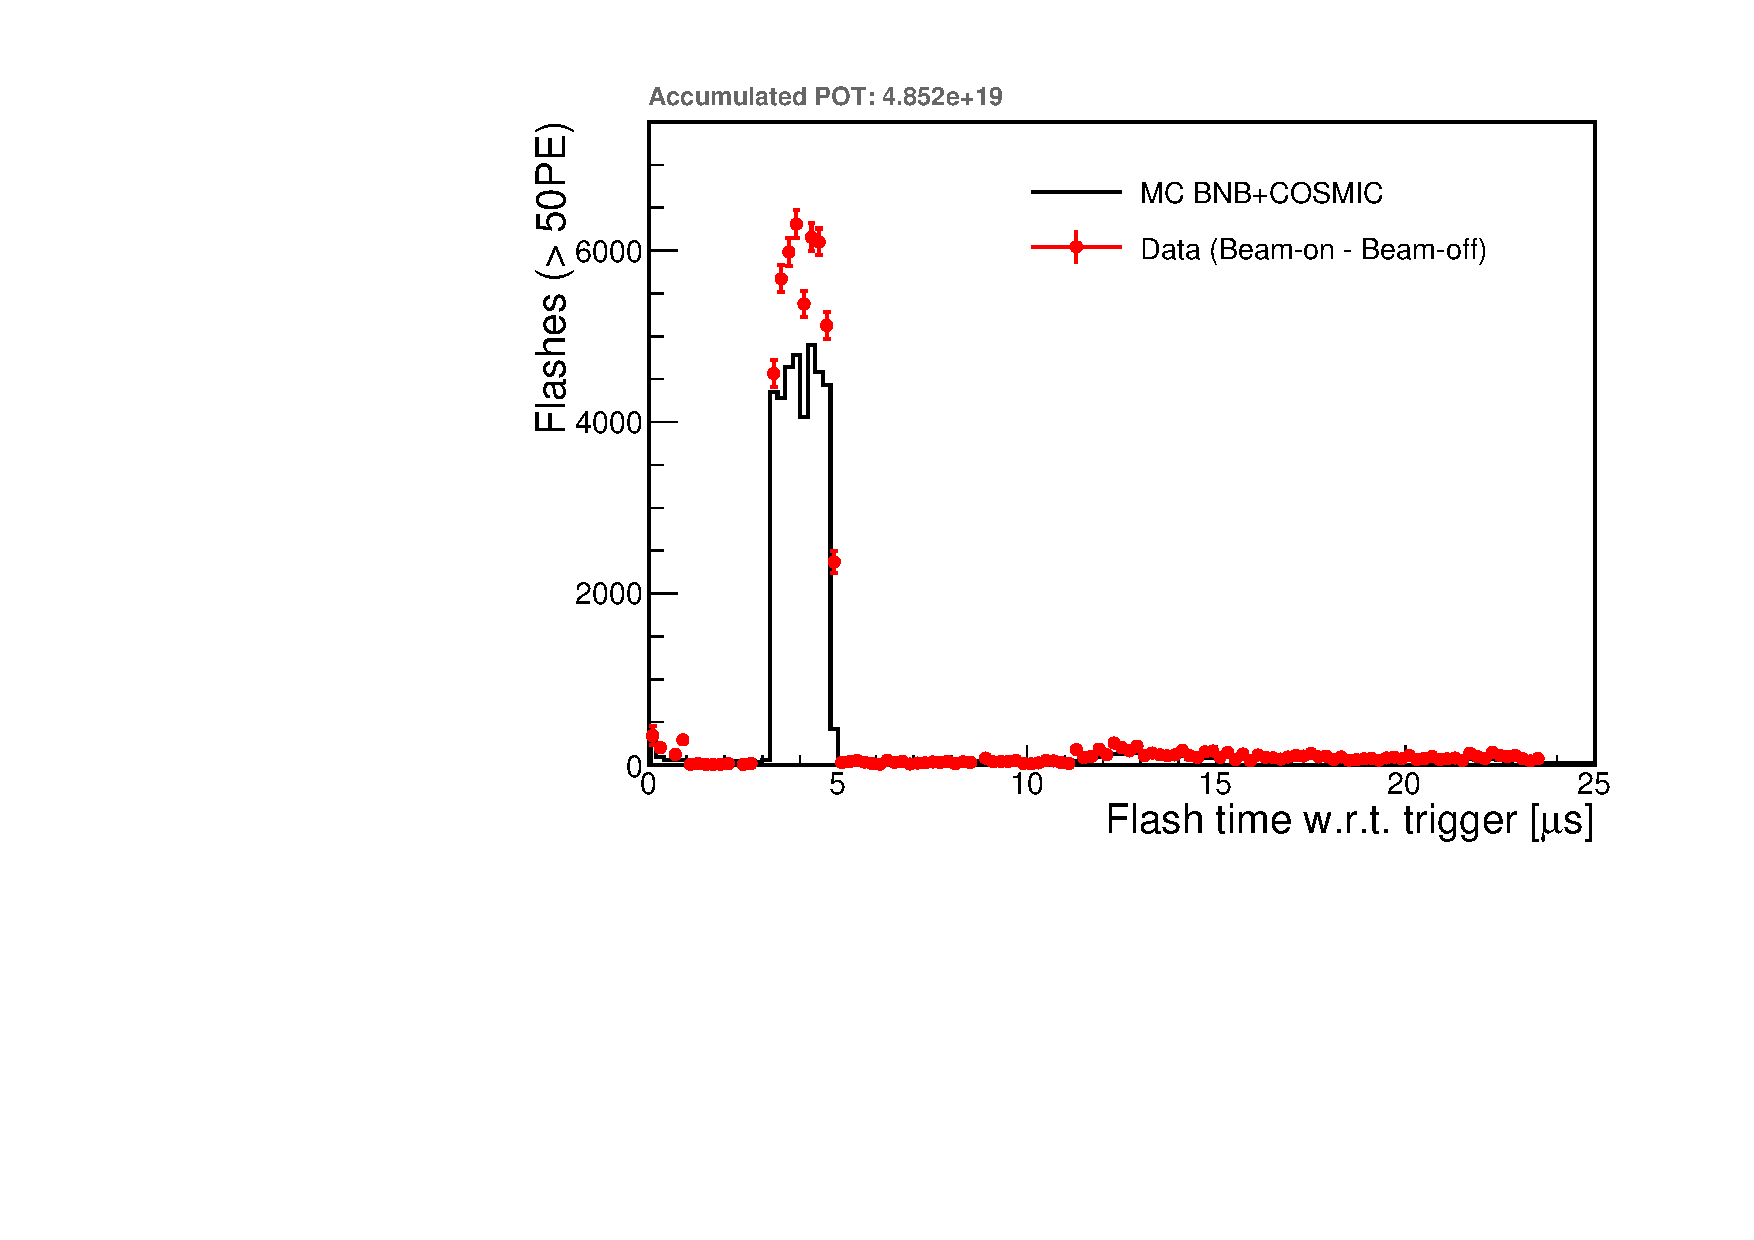
\includegraphics[width=0.98\textwidth]{fls_time}
\caption{Time-distribution of reconstructed optical flashes with a PE value of 50 or more, for a sample of BNBON triggered events. A clear excess in coincidence with the BNB spill is observable.}
\captionsetup{format=hang,labelfont={sf,bf}}
\label{fig:fls_time}
\end{figure}
%++++++++++++++++++++++++






\section{Normalisation of Corsika Cosmic Only Sample}

One should normalise the Corsika only sample to the same number of event of a \bnbcosmic sample, so that to scale it to the POT the \bnbcosmic sample correspond to.











\section{How to Dump \texttt{run} and \texttt{subrun} Numbers}
\label{sec:dump}

In \ls, the \texttt{beginSubRun} and \texttt{endSubRun} methods are called at the start and the end of a subrun respectively. These methods are called even if no events in a certain subrun passed a previously run filter, so that they allow to retrieve the correct number of run and subruns. For example, analysers can add a new tree to their ana-root output file, that is filled per subrun

\begin{mdframed}[style=exampledefault]%,frametitle={CosmicPFParticleTagger Module Settings}]
\begin{lstlisting}[label=some-code]
void UBXSec::endSubRun(art::SubRun& sr) {

  _sr_run    = sr.run();
  _sr_subrun = sr.subRun();
  
  _sr_tree->Fill();

}
\end{lstlisting}
\end{mdframed} 

In case of MC events, one can retrieve the POT per subrun direclty from the \texttt{art::SubRun}. For example, one can save the POTs per subrun in a tree (the variable here is called \texttt{\_sr\_pot}):

\begin{mdframed}[style=exampledefault]%,frametitle={CosmicPFParticleTagger Module Settings}]
\begin{lstlisting}[label=some-code]
void UBXSec::endSubRun(art::SubRun& sr) {

  art::Handle<sumdata::POTSummary> potsum_h;
  if(sr.getByLabel("generator", potsum_h)) {
    _sr_pot = potsum_h->totpot;
  }

}
\end{lstlisting}
\end{mdframed}

This TTree is going to be filled per subrun with the run and subrun number. Moreover, since this TTree will be part of the output ana-root file, the analyser will have the run and subrun numbers only for the files that passed the grid processing.
At this point one can loop over the this TTree and build a txt file with the run and subrun numbers and then call Zarko's script:\\

\texttt{/uboone/app/users/zarko/getDataInfo.py -v2 \\ -\/-run-subrun-list runsubrun\_list.txt}\\

One example to do that is by using a script like the following one, which can be found at \href{https://github.com/marcodeltutto/UBXSec/blob/master/Utils/countPOT.py}{this link}.

\begin{mdframed}[style=exampledefault]%,frametitle={CosmicPFParticleTagger Module Settings}]
\begin{lstlisting}[label=some-code, language=Python]
#!/usr/bin/env python

# usage: python countPOT.py -f /path/to/ana_*_output.root

import argparse
parser = argparse.ArgumentParser(description='Counts POT.')
parser.add_argument('-f', action='store', dest='infile',
                    help='File name (multiple files using * are ok.')

args = parser.parse_args()

import os
from ROOT import *
from glob import glob

# Opening root file
fname = glob(args.infile)
print "Input file(s): ", fname

# Creating TChain
chainPOT = TChain("UBXSec/pottree")
for f in fname: 
  chainPOT.Add(f)
           
# Printing the number of entries
entriesPOT = chainPOT.GetEntries()
print "Number of entries in the POT tree: ", entriesPOT

file = open("runsubrun_list.txt","w") 

# Getting POT number
for jentry in xrange( entriesPOT ):
  file.write("%d" % chainPOT.run)
  file.write(" ")
  file.write("%d" % chainPOT.subrun)
  file.write("\n")

file.close()

os.system('/uboone/app/users/zarko/getDataInfo.py -v2 --run-subrun-list runsubrun_list.txt')
os.system('rm runsubrun_list.txt')
\end{lstlisting}
\end{mdframed} 

In case you are running with NuMI data, it is important to change the next to last line in order to take into account the prescale factor and print the correct variables.


\renewcommand*{\bibfont}{\footnotesize}
%\nocite{*}
\printbibliography
\begin{comment}
\begin{thebibliography}{99}
\bibitem{det}{\footnotesize MicroBooNE Collaboration, {12}{P02017}{2017}}.

\bibitem{numu}MicroBooNE-Public-Note-1010 (2016) \url{http://microboone.fnal.gov/public-notes/}.

\bibitem{nc}MicroBooNE-Public-Note-1025 (2016) \url{http://microboone.fnal.gov/public-notes/}.

\end{thebibliography}
\end{comment}


\end{document}













